% \PassOptionsToPackage{gray}{xcolor}
\documentclass[a4paper,nofonts,raggedright,titlepage,openany]{tufte-book}

% \usepackage[utf8]{inputenc}
% \usepackage[T1]{fontenc}

\usepackage{ifxetex}
\usepackage{fontspec}
\setmainfont[Ligatures=TeX,Numbers=OldStyle]{Cardo}
\setsansfont[Scale=0.94]{Cabin}
\setmonofont[Scale=0.94]{Consolas}
\usepackage{fontawesome}

\newcommand\sectionnote[1]{\marginnote{\color{RubineRed}#1}}

\ifxetex
  \newcommand{\textls}[2][5]{%
    \begingroup\addfontfeatures{LetterSpace=#1}#2\endgroup
  }
  \renewcommand{\allcapsspacing}[1]{\textls[15]{#1}}
  \renewcommand{\smallcapsspacing}[1]{\textls[10]{#1}}
  \renewcommand{\allcaps}[1]{\textls[15]{\MakeTextUppercase{#1}}}
  \renewcommand{\smallcaps}[1]{\smallcapsspacing{\scshape\MakeTextLowercase{#1}}}
  \renewcommand{\textsc}[1]{\smallcapsspacing{\textsmallcaps{#1}}}
\fi

\usepackage{ragged2e}

\renewcommand{\maketitlepage}{%
  \cleardoublepage
  \begin{fullwidth}%
    \sffamily
    \RaggedRight\sloppy% <-- added this line
    \fontsize{24}{26}\selectfont\par\noindent\textcolor{darkgray}{\smallcaps{\thanklessauthor}}%
    \vspace{11.5pc}%
    \fontsize{40}{44}\selectfont\par\noindent\textcolor{darkgray}{\smallcaps{\thanklesstitle}}%
    \vfill
    \fontsize{16}{18}\selectfont\par\noindent{\thanklesspublisher}%
  \end{fullwidth}%
  \thispagestyle{empty}%
  \clearpage
}

%% Font settings suggested by fbb documentation.
% \usepackage{textcomp} % to get the right copyright, etc.
% \usepackage[lining,tabular]{fbb} % so math uses tabular lining figures
% \usepackage[scaled=.94,type1]{cabin} % sans serif in style of Gill Sans
% \usepackage[varqu,varl]{zi4}% inconsolata typewriter
% \useosf % change normal text to use proportional oldstyle figures
%\usetosf would provide tabular oldstyle figures in text

\setsidenotefont{\sffamily\footnotesize}
\setmarginnotefont{\sffamily\footnotesize}
\setcaptionfont{\sffamily\itshape\footnotesize}
\titleformat{\part}{\mdseries\huge}{\textsc{Part \thepart}}{1em}{\textsc}

\usepackage[os=win]{menukeys}
\renewmenumacro{\directory}{pathswithfolder}
\renewcommand\drawtikzfolder[1][black]{\textcolor{#1}\faFolderO{}}

\usepackage{graphicx}

\setcounter{secnumdepth}{2}
\setcounter{tocdepth}{2}
\usepackage{enumitem}
\setlist[itemize,enumerate]{noitemsep}

\usepackage[cachedir={_minted}]{minted}
\setminted[latex]{breaklines,breaksymbolleft={\phantom{\ttfamily aaaa}},bgcolor={Beige!30!white}}
\setmintedinline{bgcolor={Beige!30!white}}

\usepackage{mdframed}
\mdfsetup{backgroundcolor=Beige!30!white,hidealllines=true}
% \mdfsetup{hidealllines=true}
% \surroundwithmdframed{minted}

\usepackage{silence}
\WarningFilter{latex}{Marginpar on page}

\newsavebox{\edition}
\savebox{\edition}{\sffamily\LARGE\smallcaps{version 1.0\hspace{2em}October 20, 2015}}

\title[Guide on Using upnmthesis]{A \LaTeX\  Class \& Template for UPNM Theses\\\noindent%
\usebox{\edition}}
%{Guide on Using \texttt{upnmthesis} for Writing Universiti Pertahanan Nasional Malaysia Theses with \LaTeX}
% \subtitle{version 1.0, October 20, 2015}
\author{Lian Tze Lim, Ph.D.}
\publisher{%
\makebox[1em]{\faEnvelopeO{}}\enspace\smallcaps{liantze\string@gmail.com}\\\noindent
\makebox[1em]{\faGlobe{}}\enspace\smallcaps{http://liantze.penguinattack.org/}%
}

\begin{document}
% \usemintedstyle{bw}

\maketitle

% \begin{abstract}
\texttt{upnmthesis} is a \LaTeX\ class \marginnote{The latest version of this template can be downloaded from \url{http://liantze.penguinattack.org/latextypesetting.html\#upnmthesis}.} for authoring theses that fulfil formatting specifications required by Universiti Pertahanan Nasional Malaysia (\textsc{upnm}). This class and template was commissioned by the university's Centre of Graduate Studies in October, 2015, for both undergraduate and postgraduate theses.

A sample \directory{sample-thesis.tex}, as well as relevant sample chapters, are included in the package,\marginnote{\texttt{upnmthesis} is available as a template on Overleaf.} which I recommend you modify for your own thesis write-up. (You can rename it, but I'll stick with the file name `\texttt{sample-thesis.tex}' throughout this guide.)
% \end{abstract}

\tableofcontents

% \smallskip

\chapter{Setting Up}

\section{Compiling the Template the Easy Way}\sectionnote{\faCloud{} In the cloud!}
You may want to consider writing your thesis in the cloud, so that you won't have to maintain your own local \LaTeX{} installation or setting up the processing tools.

There are now a number of \LaTeX{} cloud editing platforms, e.g.~Overleaf, \marginnote{Disclosure: I'm the Community \TeX{}pert at Overleaf.} ShareLaTeX, Authorea, etc. The \textsc{upnm} thesis template is available on Overleaf.


\section{Configuring TeXworks to Compile \texttt{upnmthesis}}\label{sec:texworks}\sectionnote{\faGears{} Configs for TeXworks. Other editors should have something similar.}
Assuming TeXworks is your \LaTeX\ editor of choice, you will probably want to configure it so that you can process your glossary and list of own publications from within TeXworks.
You should work through this section to ensure that you are able to compile the sample thesis successfully.

(You can always, of course, opt to run the relevant commands from the command line prompt, or adapt these configurations for other editors and operating systems.)

%This section will also mention a few things to note when compiling and printing your thesis.

\subsection{Tool Configuration for Generating the List of Acronyms}\label{sec:texworks:makeglossaries}
Access the TeXworks menu \menu{Edit > Preferences > Typesetting}. Add a new processing tool called `List of Acronyms'. Configure it as shown in Figure~\ref{fig:texworks:acronyms} (p.\pageref{fig:texworks:acronyms}).

\begin{figure}
\centering
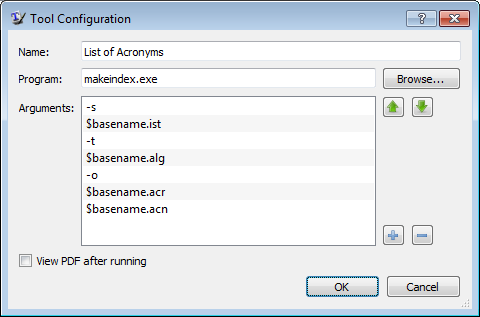
\includegraphics[width=.8\textwidth]{texworks-acronyms}
\caption{Setting up the `List of Acronyms' processing tool in TeXworks}
\label{fig:texworks:acronyms}
\end{figure}

On Linux and Mac systems, this is equivalent to the command line

\begin{fullwidth}
\begin{minted}{bash}
$  makeindex -s <basename>.ist -t <basename>.alg -o <basename>.acr <basename>.acn
\end{minted}
\end{fullwidth}

\marginnote[0.5em]{where \texttt{<basename>} is the name of your main file (i.e.~\texttt{sample-thesis}).}


\subsection{Tool Configuration for Generating the List of Publications}
Add another processing tool called ``Publication List''. Configure it as shown in Figure~\ref{fig:texworks:publist} (p.~\ref{fig:texworks:publist}).
On Linux and Mac systems, this is equivalent to the command line

\begin{minted}{bash}
$  bibtex own
\end{minted}

\begin{figure}
\centering
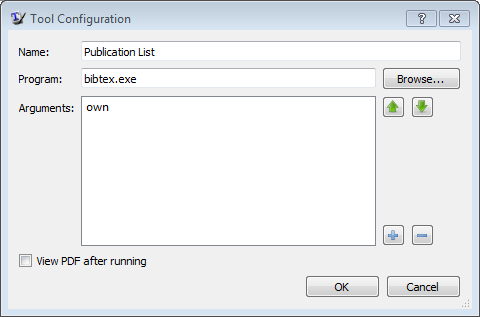
\includegraphics[width=.8\textwidth]{texworks-publist}
\caption{Setting up the `Publication List' processing tool in TeXworks}
\label{fig:texworks:publist}
\end{figure}



\subsection{Compiling \texttt{thesis.tex}}\sectionnote{\faCode{} Compilation steps}
When using TeXworks, the processing tools should be run on \texttt{thesis.tex} in the following sequence: 
\begin{enumerate}
\item pdfLaTeX + BibTeX + Makeindex \marginnote{You will need to run `List of Acronyms' again if you add and use a new acronym. Similarly, run `Publication List' again if you add a new self publication. Don't forget to run `pdfLaTeX + BibTeX + Makeindex' after that!}
\item List of Acronyms
\item Publication List
\item pdfLaTeX + BibTeX + Makeindex
\end{enumerate}

\subsection{Why is there a blank page before the title page and at the end?!}\sectionnote{\faQuestion\faExclamation{} What, blank pages?!}
The thesis preparation guidelines say there needs to be a blank page between the cover and the title page, and another at the very end, so \textsf{umalayathesis} forces one just in case you forgot to insert one. \faSmileO

\subsection{Printing from Acrobat Reader}\sectionnote{\faPrint{} Make sure the print out isn't shrunk!}
Remember to set the \textbf{paper size} to \textbf{A4} and \textbf{page scaling} to \textbf{None} in the \textsf{Print} dialog, otherwise the margins would be incorrect.


\chapter{Using the Template}

We'll now look at how you can modify the template \LaTeX{} files to suit your own thesis.

\section{Document Class Options}

To `activate' the class, make sure your main document file (e.g.~\texttt{sample-thesis.tex}) starts off with \mintinline{latex}{\documentclass{upnmthesis}}. This will set up the page margins, paragraph spacing, indents, page numbers, font face and size, content list and section headings, citation and bibliography format, amongst other things.


There are three options \marginnote{All three options are off as default.} that you can pass to the document class declaration:

\begin{description}
\item[\ttfamily undergrad]   
If you're writing an undergraduate thesis. \marginnote{Remember to specify
             your \mintinline{latex}{\faculty} if using this option.} There will then
             be no exam committee approval, even if you have specified
             \texttt{examcommapproval} -- see section~\ref{sec:approval}. and the wordings of the supervisory
             committee approval will be different.
%
\item[\ttfamily newtx]     Loads the \texttt{newtxtext} and \texttt{newtxmath} font packages if these
             packages are installed; they have nicer math fonts.
             Otherwise \texttt{mathptmx} will be loaded as default.
%
\item[\ttfamily microtype] Even nicer typographic output! Reduces chances of hyphenation
             but \emph{sometimes} (though rare) may cause an endless loop as
             the typesetting engine tries to find an optimal line break.
\end{description}


\section{List of Abbreviations}
\label{sec:list:abbrevs}

To facilitate automatic sorting and expansion of abbreviations, \texttt{upnmthesis} uses the \texttt{glossaries} package. Preferably, the list of abbreviations and symbols are defined in a separate \directory{myacronyms.tex}, and included in the thesis just after \mintinline{latex}{\begin{document}}:

\begin{minted}{latex}
%!TEX ROOT=sample-thesis.tex

%% Format: \newacronym{label}{abbreviated form or symbol}{full form}
\newacronym{LI}{LI}{lexical item}
%% need to specify plural forms explicitly, otherwise will be
%% auto-genetared as "part of speechs"
\newacronym[firstplural={parts of speech (POS)},plural={POS}]%
{POS}{POS}{part of speech}
\newacronym{NLP}{NLP}{Natural Language Processing}
\newacronym{theta}{$\theta$}{temperature degree}
\newacronym{IR}{IR}{Information Retrieval}
\newacronym{WWW}{WWW}{World Wide Web}

\end{minted}

\directory{myacronyms.tex} can contain abbreviation/acronym definitions that take the form of\\\mintinline{latex}{\newacronym{label}{abbreviated form or symbol}{full form}}:

\begin{minted}{latex}
\newacronym{LI}{LI}{lexical item}
%% need to specify plural forms explicitly, otherwise
%% will come out as "part of speechs"
\newacronym[firstplural={parts of speech (POS)}, plural={POS}]{POS}{POS}{part of speech}
\newacronym{NLP}{NLP}{Natural Language Processing}
\newacronym{theta}{$\theta$}{temperature degree}
\end{minted}

Only abbreviations that are actually called in the main text \marginnote{section \ref{sec:texworks:makeglossaries}} via \mintinline{latex}{\gls} and related commands,will be printed \marginnote{\mintinline{latex}{\printacronyms}, section \ref{sec:content:lists}} in the List of Abbreviations.

\section{Front Matter}

\mintinline{latex}{\frontmatter} marks the start of the thesis front matter -- i.e.~everything before your first chapter. This includes the cover page, title page, dedication (optional), acknowledgements, English and Malay abstracts, approval forms, declaration form, and content lists.

\subsection{Information about Your Thesis}

Modify the following lines in the template to suit your own thesis. These information will be used to generate the cover and title pages, as well as various forms in the thesis. Don't forget to specify your \mintinline{latex}{\faculty}  if you have specified the \texttt{undergrad} document option.

\begin{minted}{latex}
\author{Your Name}
\title{Your Thesis Title}
\degree{Your Degree (e.g. Doctor of Philosophy)}
\studyfield{Computer Science}

%% If Bachelor programme, you'll need to uncomment
%% and specify the following line
% \faculty{Faculty of Engineering}
\submissionyear{2011}
\submissionmonth{October}
\vivadate{25 August 2011}
\end{minted}


\subsection{Cover and Title Pages}

\mintinline{latex}{\makecoverandtitlepage} generates the cover page, \marginnote{The `cover page' is the hard cover, while the title page is printed on a plain A4 paper.} a blank page, and then the title page, using the information you've provided.

\subsection{Dedication \& Acknowledgements}

You can create an optional dedication page with \marginnote{Dedications are usually short.}

\begin{minted}{latex}
\dedication{To my parents.}
\end{minted}

On the other hand, the acknowledgements section is likely to be longer -- so I've put it in \directory{acknowledgements.tex} as a sample:

\begin{minted}{latex}
\begin{acknowledgements}
Thanks guys. I owe you many.
\end{acknowledgements}
\end{minted}

\subsection{Abstracts}

Write your abstracts in separate files \marginnote{\directory{sample-abstract.tex} for the English abstract and \directory{sample-msabstract.tex} for the Malay abstract in this example}. These files do not need to contain any headings -- only the abstract text is needed.

Include them in \directory{sample-thesis.tex} like this:

\begin{minted}{latex}
\abstractfromfile{sample-abstract}
\msabstractfromfile{sample-msabstract}
\end{minted}



\subsection{Approval and Declaration Forms}
\label{sec:approval}

If you are writing a postgraduate thesis (default mode), you will need two approval forms: one from the \emph{Examination Committee}, and one from the \emph{Supervisory Committee}. Examination Committee approval is \marginnote{i.e.~if you used \texttt{undergrad} class option.} not required for undergraduate theses.

To produce the Examination Committee approval form, you'll need to specify the committee \mintinline{latex}{\member}s (Chairman, the two Internal Examiners and the External Examiner) in the \mintinline{latex}{examcommapproval} environment: \marginnote{The \texttt{examcommapproval} environment will be ignored if you have specified the \texttt{undergrad} class option.}

\marginnote{Default values for \mintinline{latex}{\member} keys, if you do not explicitly define them:
\begin{description}[noitemsep]
\item[\ttfamily title] (empty)
\item[\ttfamily department] (empty)
\item[\ttfamily institute] Universiti Pertahanan Nasional Malaysia
\item[\ttfamily role] Member
\end{description}
}


\begin{minted}{latex}
\begin{examcommapproval}
  % Exam Committee Chairman
  \member[title=Professor,                        department={Faculty of Mathematics},                                  role={Chairman}]
  {Name of Chairperson, PhD}
  % Internal Examiner 1
  \member[title=Associate Professor,                         department={Faculty of Engineering},                  role={Internal Examiner}]{Name of Examiner 1, PhD}
  % Internal Examiner 2
  \member[title={},                        department={Faculty of Engineering},              role={Internal Examiner}]{Name of Examiner 2, PhD}
  % External Examiner
  \member[title=Associate Professor,                  department={School of Chemical Engineering},                institute={Imperial College},               role={External Examiner}]{Name of External, PhD}
\end{examcommapproval}
\end{minted}

The Supervisory Commitee approval \marginnote{The wording for Supervisory Commitee approval will be generated differently for postgraduate and \texttt{undergrad} theses.} is created in a similar manner, using the \mintinline{latex}{supervisoryapproval} environment.

\begin{minted}{latex}
\begin{supervisoryapproval}
  % Supervisory Committee Chairman
  \member[title={Associate Professor},             role={Chairman},                           department={Faculty of Engineering}]
    {Name of Chairperson, PhD}
  % Supervisory Committee Member 1
  \member[title={Ir.}, department={Faculty of Engineering}]{Name of Member 1, PhD}
  % Supervisory Committee Member 2
  \member[department={Faculty of Engineering}]
    {Name of Member 2, PhD}
\end{supervisoryapproval}

\end{minted}

\mintinline{latex}{\declarationpage
} generates the thesis declaration page. Remember to get all these pages signed before submission.

\subsection{Content Lists}
\label{sec:content:lists}

The table of contents, list of tables, list of figure, list of appendices  and list of abbreviations are generated by the following lines.

\begin{minted}{latex}
{\clearpage\SingleSpacing
\tableofcontents*\clearpage
\listoftables\clearpage
\listoffigures\clearpage
%% Comment out the following line if you have two or 
%% less appendices
% \listofappendices\clearpage
\printacronyms\clearpage
}
\end{minted}

Note that you should leave \mintinline{latex}{\listofappendices} commented if you have two or less appendices. \marginnote{A single item `Appendices' will then be added to the table of contents.} Conversely, \marginnote{If \mintinline{latex}{\listofappendices} is issued, the item `Appendices' will not appear in the table of contents.} if you have three appendices or more, you should uncomment it, so that a separate list of appendices can be generated.


\section{Main Chapters}

I highly recommend that each chapter be written in a separate file. For example, \directory{sample-chap-intro.tex} may have the contents  \marginnote{The \mintinline{bash}{!TEX ROOT} directive
indicates to TeXworks (and also TeXshop on the Mac) that \directory{sample-chap-xxx.tex} are `sub-files' of \directory{thesis.tex}.

This means if you hit \keys{Ctrl+T} when you  are editing \directory{chap-xxx.tex}, \directory{sample-thesis.tex} will get compiled instead.}


\begin{minted}{latex}
%!TEX ROOT=sample-thesis.tex
\chapter{Introduction}
This is the introduction chapter.

\section{Problem Background}
We study the...
\end{minted}

And \directory{sample-chap-litreview.tex}:

\begin{minted}{latex}
%!TEX ROOT=sample-thesis.tex
\chapter{Literature Review}
We review the state of the art in...

\section{Early Approach}
Researchers first attempted to...
\end{minted}


In \directory{sample-thesis.tex}, these chapter files are included with the following lines:

\begin{minted}{latex}
\mainmatter         % signal start of main chapters
%!TEX ROOT = sample-thesis.tex
\chapter{Introduction}

So this is the preamble at the beginning of the chapter. The purpose may be to introduce the themes of the chapter and main headings.

See how inter-paragraph spacing is larger. \lipsum[3]

\section{First Test and I need a really long title, please do oblige me won't you? Just a few more words and yes we're there}
\lipsum[1-2]

\begin{figure}[hbt!]\centering
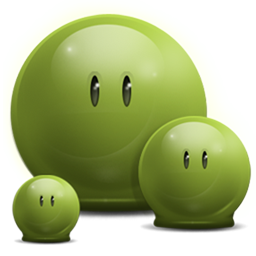
\includegraphics[width=.3\textwidth]{green}
\caption{First figure. OK?}
\end{figure}

\begin{figure}[hbt!]\centering
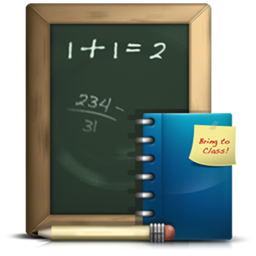
\includegraphics[width=.3\textwidth]{school}
\caption{Second figure. Now I need a long caption to test out how things look in the List of Figures. Is this long enough yet? Is it? Is it?}
\end{figure}


\begin{figure}[hbt!]
\centering
%
\begin{minipage}{0.3\textwidth}
\centering
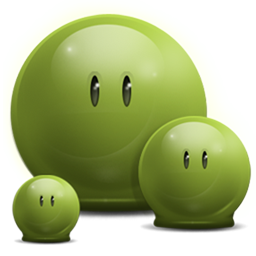
\includegraphics[width=\linewidth]{green}
\subcaption{The first subfigure}
\end{minipage}
%
\hspace{1cm}
%
\begin{minipage}{0.3\textwidth}
\centering
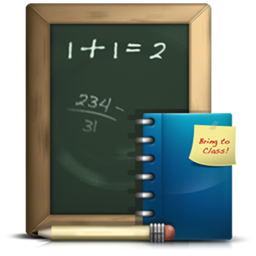
\includegraphics[width=\linewidth]{school}
\subcaption{The second subfigure}
\end{minipage}

\caption{An example with subfigures}
\end{figure}

\begin{subsecs}
\subsection{Second Test}
Their \cite{audibert:2004} requirements\footnote{See here, how weird, how to fill out an entire line. See here, how weird, how to fill out an entire line. See here, how weird, how to fill out an entire line. See here, how weird, how to fill out an entire line. See here, how weird, how to fill out an entire line. } are really amazing\footnote{don't you agree?} \cite{budanitsky:hirst:2006}.

Looks like everyting's working. Great. Let's talk about \glspl{LI} and \glspl{POS} in \gls{NLP}. I mention again \glspl{LI}. Oh I have a symbol too, it's \gls{theta}.

\subsection{This is another Subsection}

Remember that subsections need to be indented! 

\end{subsecs}

\section{Yeah}

And here's a long quotation, it should be an indented block and single-spaced:

\begin{quotation}
\lipsum[5]
\end{quotation}

Time for some maths, and later there's a table.

\begin{equation}
\left[M\frac{\partial }{\partial M}+\beta(g)\frac{\partial }{\partial g}+n\gamma\right] G^{(n)}(x_1,x_2,\ldots,x_n;M,g)=0
\end{equation}

\begin{table}[hbt!]
\caption{This is a table}
\centering
\begin{tabular}{ l c r }
\hline
Hey & How's it & Going?\\ \hline
Fine! & Just great. & See ya!\\
Fine! & Just great. & See ya!\\
\hline
\end{tabular}
\end{table}

\lipsum[7-12]
\input{sample-chap-litreview}
\input{...}
\end{minted}


\subsection{Typesetting the Text}

Sections, subsections, graphics files, figures, tables, itemize and enumerated lists, etc are created using the standard \LaTeX{} commands. See \directory{sample-chap-intro.tex} for some examples, including how to create subfigures (and by extension, subtables).


\subsection{About Subsections}

Subsections need to be indented, so remember to surround your subsections with \mintinline{latex}{\begin{subsecs}...\end{subsecs}} like this:

\begin{minted}[escapeinside=||]{latex}
\section{Discussion}
We will highlight...

\begin{|\bfseries\color{red}subsecs|}
\subsection{First Issue}
...
\subsection{Second Issue}
...
\end{|\bfseries\color{red}subsecs|}

\section{Next section}
...
\end{minted}


\subsection{Citatons and Bibliography}

Citations and bibliography are done using Bib\TeX{}, adopting the \smallcaps{APA} style. Both \texttt{natbib} and \texttt{apacite} commands can be used -- in most cases you'll just need the following:

\begin{fullwidth}
\begin{tabular}{l @{\enspace$\longrightarrow$\enspace} l}
\mintinline{latex}{\cite{John:2004}} & John (2004)\\
\mintinline{latex}{\citep{John:2004}} &(John, 2004)\\
\mintinline{latex}{\citet{John:2004}} & John (2004)\\
\mintinline{latex}{\citep[p.5]{John:2004}} & (John, 2004, p.5)\\
\mintinline{latex}{\citep[see also][p.5]{John:2004}} & (see also John, 2004, p.5)\\
\mintinline{latex}{\citeauthor{John:2004}} & John\\
\mintinline{latex}{\citeyear{John:2004}} & 2004\\
\end{tabular}
\end{fullwidth}

\subsection{Calling Abbreviations}
\label{sec:abbrevs:gls}

Use \mintinline{latex}{\gls} and related commands to call abbreviations that you previously defined \marginnote{section \ref{sec:list:abbrevs}} in \directory{myacronyms.tex}. On first mention, the full form will be displayed, and on subsequent mentions, the short form will be used. For example:

\begin{tabular}{l @{\enspace$\longrightarrow$\enspace} l}
\mintinline{latex}{\gls{LI}} (first use) & lexical item (LI) \\
\mintinline{latex}{\Gls{LI}} (first use) & Lexical item (LI) \\
\mintinline{latex}{\glspl{LI}} (first use) & lexical items (LIs) \\
\mintinline{latex}{\gls{LI}} (subsequent uses) & LI \\
\mintinline{latex}{\glspl{LI}} (subsequent uses) & LIs \\
\mintinline{latex}{\glspl{POS}} (first use) & parts-of-speech (POS)
\end{tabular} \marginnote{A custom plural form was specified for POS, so we get `parts-of-speech' instead of `part-of-speech'}

Note that only abbreviations that have actually been used via \mintinline{latex}{\gls} etc will appear in the List of Abbreviations.

\section{Back Matter}

The back matter starts when the final main chapter has ended. It consists of the bibliography, appendices, publication list and  biodata. \emph{However note that the \mintinline{latex}{\backmatter} command \emph{should not} be used.}

\subsection{Bibliography}

The bibliography file is a standard Bib\TeX{} \texttt{.bib} file -- a standard \mintinline{latex}{\bibliography{sample}} is sufficient.

\subsection{Appendices}

Similar to the main chapters, it is recommended to put each appendix in its own file.

\begin{minted}{latex}
\begin{appendices}
%!TEX ROOT = sample-thesis.tex
\chapter{Manuals, Technical Specifications, Documentations, Example Scenarios}

%!TEX ROOT = sample-sample.tex
\chapter{Try}

\lipsum[1-2]

\end{appendices}
\end{minted}

\subsection{Biodata}
Write your personal biodata in the \mintinline{latex}{biodata} environment. This can go into a separate \directory{biodata.tex}, which is later \mintinline{latex}{\input}-ed.

\begin{minted}{latex}
\begin{biodata}
Put your personal biodata as required here.
\end{biodata}
\end{minted}

\subsection{Publication List}

First, make sure that you enter details about your own publications in your Bib\TeX{} file, \directory{myrefs.bib} file.
\marginnote{You can list your publications in a different \texttt{.bib} file -- just remember to pass in the correct file name to \mintinline{latex}{\bibliographyown}.}
Then in \directory{sample-thesis.tex}, list the keys of your publications in \mintinline{latex}{\nociteown}, and display the publication list using \mintinline{latex}{\bibliographyown}:

\begin{fullwidth}
\begin{minted}{latex}
\nociteown{Lim:2009,Bond:etal:WordNetBahasa:2014,Lim:etal:2014,Lim:etal:acl:lookup}
\bibliographyown{myrefs}
\end{minted}
\end{fullwidth}

The publication list sorts entries according to the \smallcaps{APA} requirements by default, i.e.~based on the first authors' last names. This may not be what you want, e.g.~you may want to sort your publications chronologically. In this case, we can force \smallcaps{APA} to sort by a custom key, using the \mintinline{latex}{\APACSortNoop} command. For example, the following will sort by chronological order of the publication date:

\marginnote{Note that the \mintinline{latex}{\APACSortNoop} command should be placed just before the \emph{last name} of the first author.

You may define the custom value differently if you want to sort by reverse chronological order.}

\begin{minted}{latex}
@ARTICLE{Bond:etal:WordNetBahasa:2014,
  author={{\APACSortNoop{2014}}Bond, Francis and Lim, Lian Tze and Tang, Enya Kong and Riza, Hammam},
  year={2014},
  ...
}

@INPROCEEDINGS{Lim:etal:acl:lookup,
  author = {{\APACSortNoop{2013}}Lim,Lian Tze and Lay-Ki Soon and Tek Yong Lim and Enya Kong Tang
  and Bali Ranaivo-Malan\c{c}on},
  year = {2013},
  ...
}

@ARTICLE{Lim:etal:2014,
  author = {{\APACSortNoop{2014}}Lim, Lian Tze and Soon, Lay-Ki and Lim, Tek Yong and Tang, Enya Kong
  and Bali Ranaivo-Malan\c{c}on},
  year = {2014},
  ...
}
\end{minted}

\nobibliography*
\bibliography{../myrefs}

\end{document}